% first section should be classic supervised auto-encoder and maybe paris auto-encoder. then the next section can be dan stowells thing, and then finally the curro-net.
In the following sections, we detail all considered shallow network architectures. Note that these network architectures can easily be extended to deep networks by adding corresponding encode and decode layers before and after the latent representation, respectively. These networks can be trained using the various inputs detailed in Chapter 3. However, for the purposes of presenting first results, we consider single FFT frames only to compare networks. %In other words, we take overlapping frames of an audio signal $y[n]$ and pass their magnitude spectrum values $Y[k]$ into our network. The signal estimate $\hat{x}[n]$ is computed by taking the IFFT and using overlap-add reconstruction by combining the magnitude spectrum estimates with the original noisy phase:

% \begin{equation}
% \hat{X_i}[k] =
% \end{equation}

\subsection{Supervised Autoencoder}

We adopt the shallow supervised autoencoder from \cite{liu2014experiments}. Used for supervised denoising, we adopt the relative network size as well as their modified nonlinear activation function. The network structure is a single hidden layer, dense neural network. In other words, we can represent our network output $\hat{X_i}[k]$ for various overlapping frames $i=1,\cdots,N$ by the following:


\begin{align}
\hat{X_i}[k] &= f_1 \big( \vec{W}^{(1)} \vec{h}_i^{(0)} + \vec{b}^{(1)} \big)\\
\vec{h}_i^{(0)} &= f_0 \big( \vec{W}^{(0)} Y_i[k] + \vec{b}^{(0)} \big)
\end{align}


This network is trained to estimate the various layer weight matrices $\vec{W}^{(l)}$ and layer bias vectors $\vec{b}^{(l)}$.

Since we are estimating a magnitude spectrogram for values in the interval $[0,\infty)$, we use a nonlinear activation function whose support is on the same interval. A natural choice is the rectified linear unit (ReLU). However, as detailed in \cite{liu2014experiments}, the ReLU is subject to a 0-derivative for negative values. The modified ReLU used in \cite{liu2014experiments}, which we denote as mReLU, is given by the following:

\begin{equation}
f(x) =
    \begin{cases}
        \hfill x \hfill & \text{if $x \ge \epsilon$}\\
        \hfill \dfrac{-\epsilon}{x-1-\epsilon} & \text{if $x < \epsilon$}
    \end{cases}
\end{equation}

The choice of $\epsilon$ used in \cite{liu2014experiments} is $10^{-5}$. This modified ReLU allows for nodes to escape zero state since the derivative is always positive. An example plot of the nonlearity is given in \ref{fig:mrelu}.

\begin{figure}[!ht]
\centering
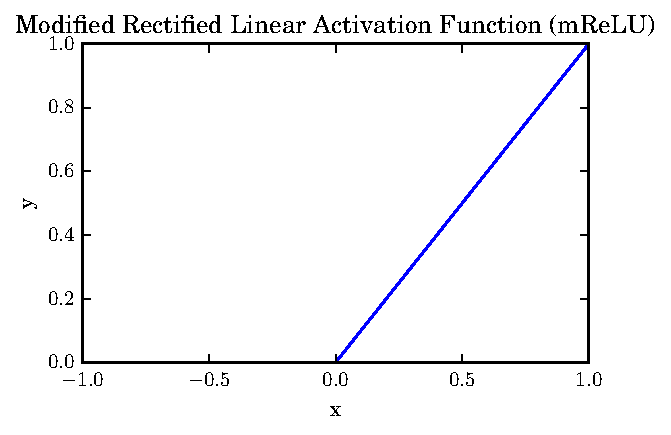
\includegraphics[width=.8\textwidth]{mrelu}
\caption[Modified Rectified Linear Unit Activation]{Modified Rectified Linear Unit Activation Function Plot}
\label{fig:mrelu}
\end{figure}

Since this network is supervised, we allow the training access to the original magnitude spectra $X[k]$. The loss function for training this network is defined as the mean squared error (MSE) between the network output and the clean spectra $X[k]$:

\begin{equation}
l(\vec{X},\vec{\hat{X}}) = \norm{\vec{X}-\vec{\hat{X}}}^{2}
\end{equation}

For our simulations, we also apply batch normalization at the input to help train more quickly and efficiently.

\subsection{Partitioned Autoencoder}

Adopted from \cite{stow}, the partitioned autoencoder is a variation of a traditional autoencoder in which we do not know the noise corruption process or the underlying clean signals directly. This model more closely models a practical scenario. Since we don't have access to clean data, we rely instead on a ``soft'' label indicating whether we have a ``noise-only'' training example or a ``noisy'' training example which possibly has the desired signal present within it.

Depending on a number of factors, a traditional autoencoder can learn many different latent representations which ultimately learn to encode and decode the underlying clean signal. A partitioned autoencoder seeks to use regularization during training to give explicit meaning to the latent variables in the network. If we can identify noise-only components in our training data, we can potentially train the network to put noise-only information into one part of the latent space. Then, the rest of the latent variables should correspond to signal-only if a sufficient representation of the noise is learned. At inference time, we can then zero out the noise-only latent variables to accomplish denoising.

In \cite{stow}, they use the following loss function to accomplish effective partitioning:

\begin{equation}\label{eq:stowloss}
l(\vec{Y}, y) = \norm{ \vec{Y} - \vec{\hat{X}}}^{2} + \dfrac{\lambda y}{\bar{\vec{C}}} \norm{\vec{C} \odot f(\vec{Y})}^{2}
\end{equation}

where $\vec{\hat{X}}=g(f(\vec{Y}))$, the latent variables are given by $f(\vec{Y})$, $\vec{C}$ is a masking matrix dependent on the minibatch and latent sizes taking on the value 1 for signal latents and 0 for noise or background latents. $y$ corresponds to the aforementioned soft label which has value 0 for a signal-plus-noise example and 1 for a noise-only example. $\lambda$ is a regularization coefficient which is set to a higher value than normally used for regularization to enforce zeroing out of signal-based latents for noise-only examples.

In other words, when we train the network, we use minibatches with fixed ordering corresponding to the same proportion of signal-plus-noise examples and noise-only examples such that $\vec{C}$ does not change on each training iteration. An example $\vec{C}$ is given in Figure \ref{fig:cmat}. For signal-plus-noise examples, the regularization term is 0, and the network seeks to reconstruct the noisy example. However, for noise-only examples, the network tries to put all of the latent energy into the pre-determined noise-only latent variables. In \cite{stow}, they balance this by choosing 25\% of minibatches to be noise-only as well as 25\% of latent variables to be noise-only.

\begin{figure}[!ht]
\centering
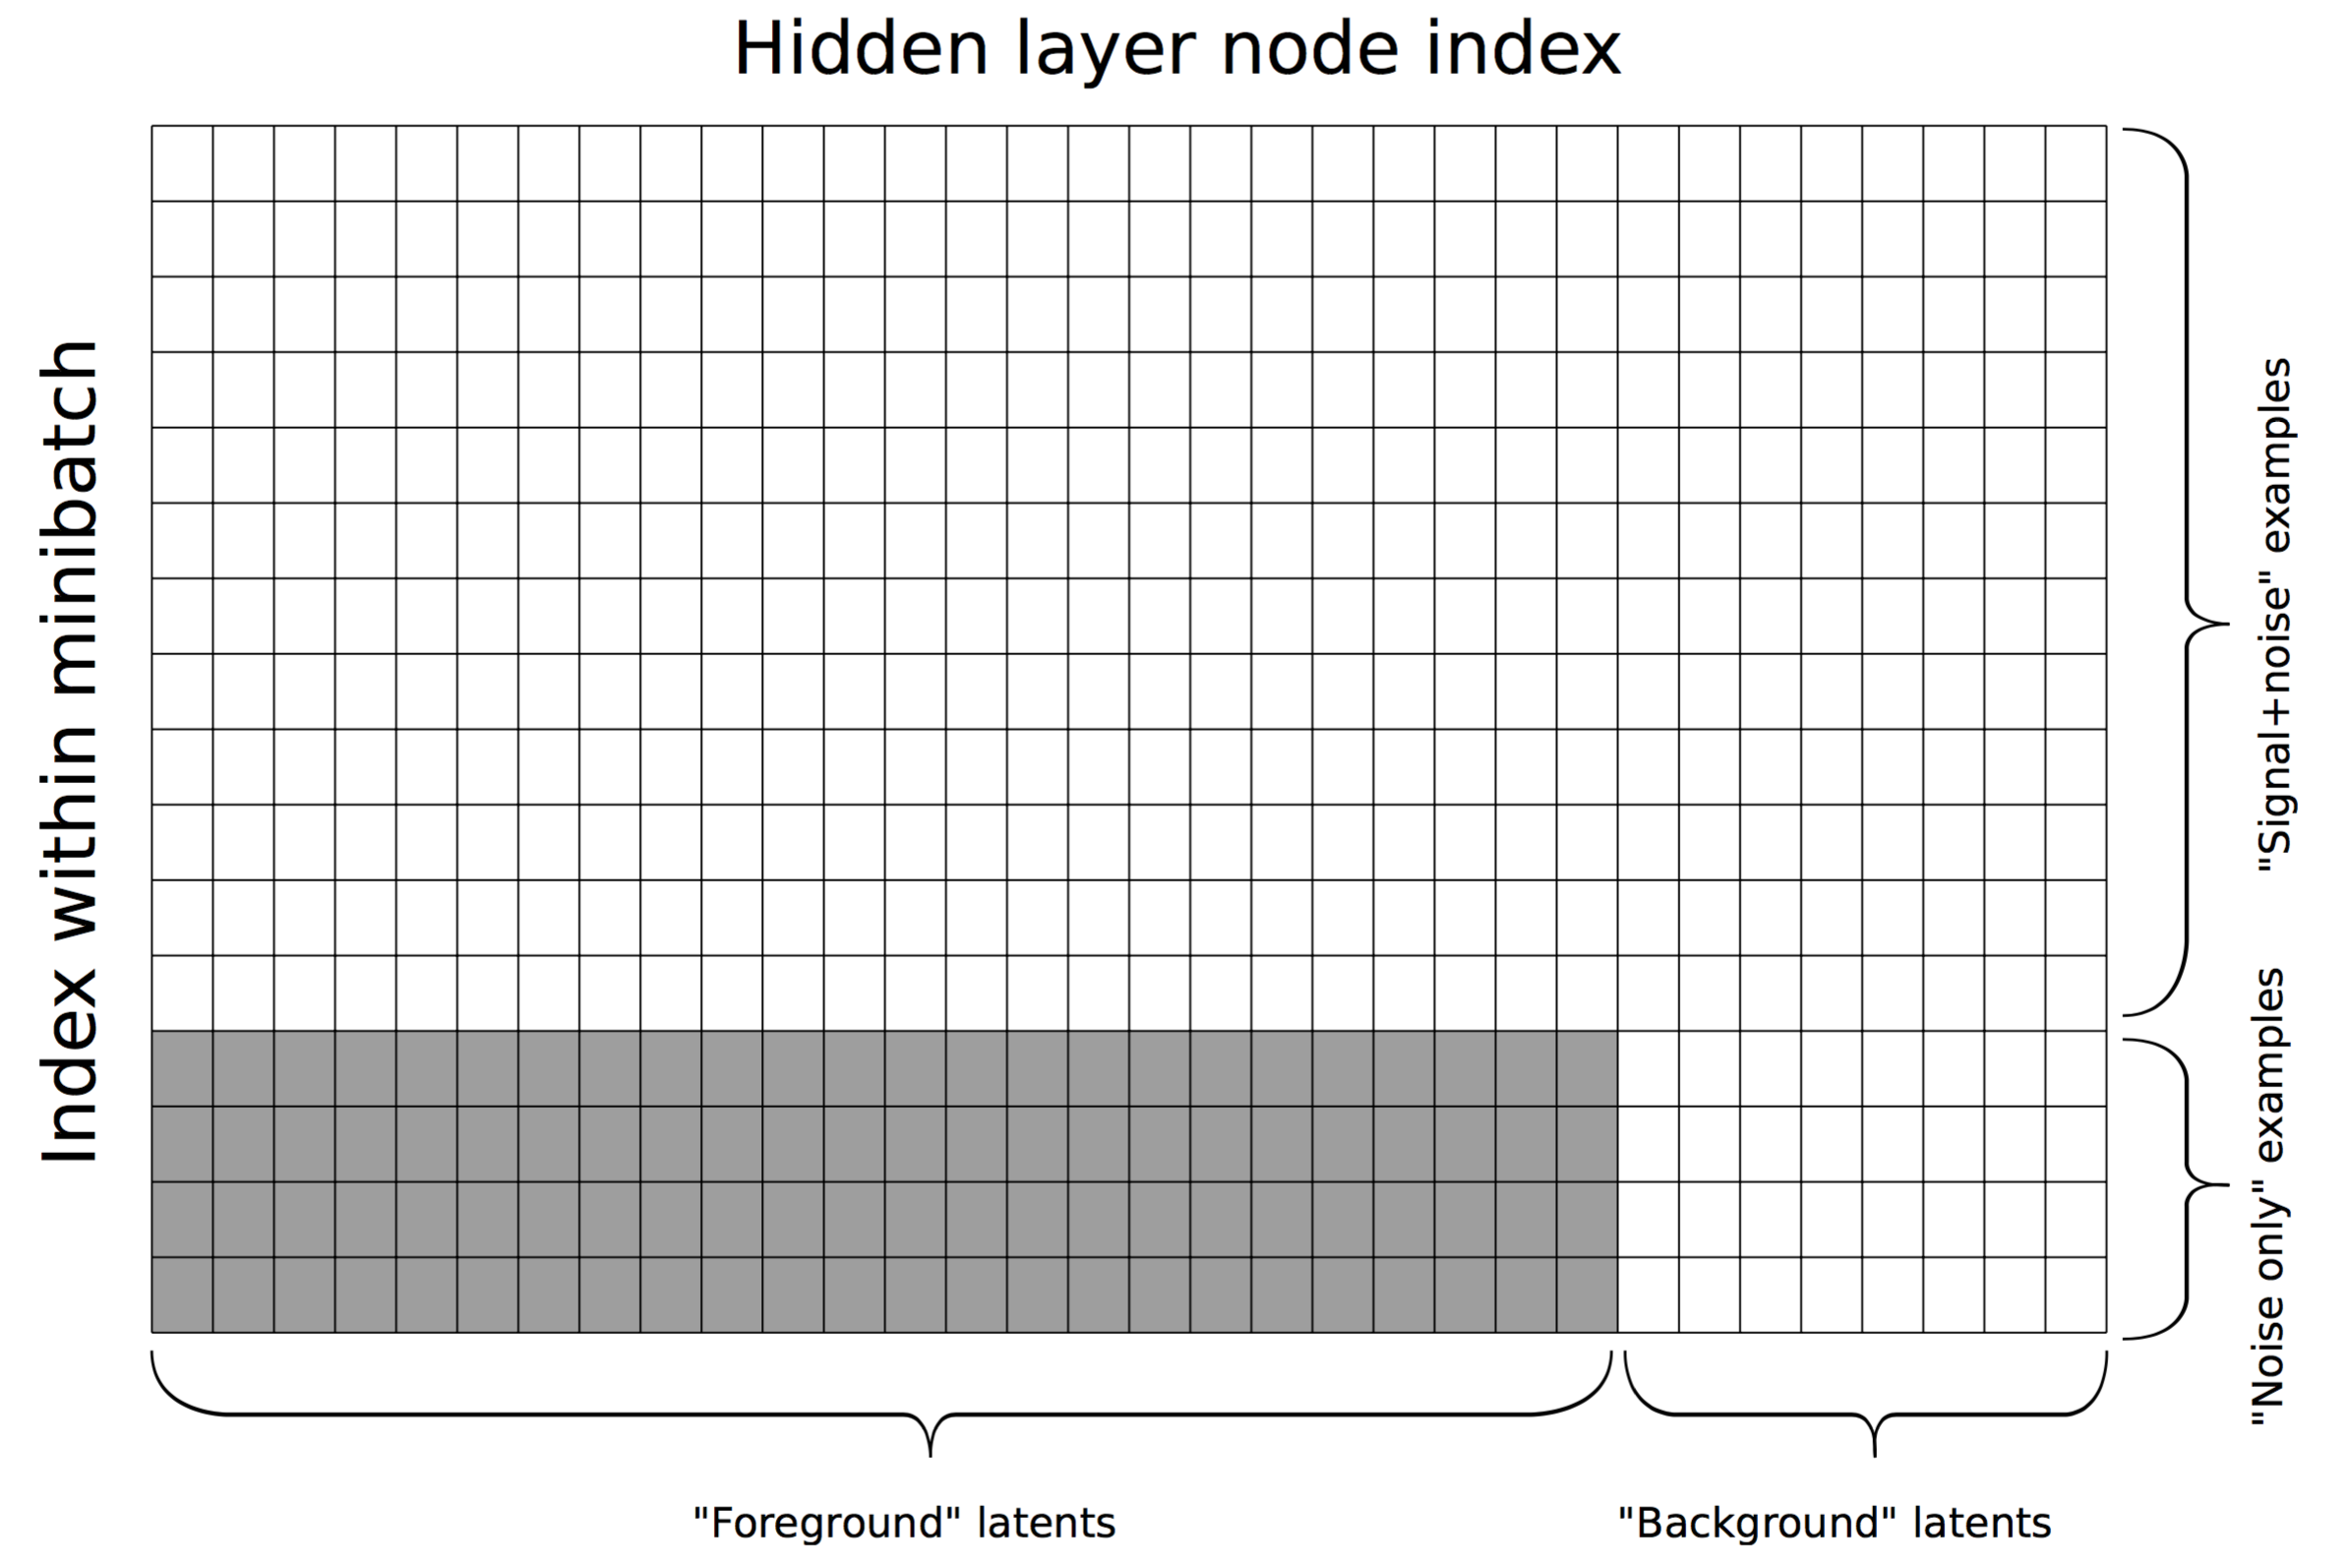
\includegraphics[width=.8\textwidth]{cmat}
\caption[Example Partitioned Masking Matrix]{Example Partitioned Masking Matrix. \cite{stow} The gray area corresponds to signal (foreground) latents for noise-only examples. We want to penalize the network for any nonzero energy in the signal latents when there are noise-only examples.}
\label{fig:cmat}
\end{figure}

Note that it is okay for noise-only examples to be mislabeled as signal-plus-noise, but the opposite would cause the signal to be misrepresented as noise. Therefore, the soft labeling of examples should be cautious on the side of labeling as noise-only.

In \cite{stow}, they use spectrogram frames as input. Their partitioned autoencoder is constructed as a shallow two-dimensional convolutional autoencoder with input normalization to zero-mean and unit-variance, maxpooling along the time index, and a ReLU nonlinearity before the latent layer. Their convolutional layer is constructed such that the frequency space is fully connected, and the convolution happens in time. The results of their autoencoder are presented in the frequency domain only, so we seek to adapt the partitioning concept to also recover cleaner time-domain audio.

Therefore, we use the same loss function as defined in Equation \ref{eq:stowloss}, but we use single magnitude spectrum frames and compare results on the mean squared error in the time-domain rather than in the frequency domain as their results presented. We also used the modified ReLU as presented from \cite{liu2014experiments}.

\subsubsection{Phase Reconstruction}

By extension, we combine the estimated magnitude spectra at the output with the original noisy phase. We can then recover a time-domain estimate of our desired signal using overlap-add resynthesis.

Other experiments we tried involved trying to explicitly or implicitly estimate the clean phase. One such explicit experiment involved training a parallel partitioned autoencoder with modified nonlinearities that tried to learn a clean phase representation. However, this ended up with a worse MSE and distorted the signal than using the original noisey phase. An implicit phase estimation example involved training the network using two channels as feature maps, where the real part of the frequency spectrum made up one feature map and the imaginary part of the frequency spectrum made up the other. This also resulted in worse reconstructed signals than the case where we estimate the magnitude spectrum and combine with the noisy phase. Sample code is provided in the appendix.

\subsection{Curro Autoencoder}

We present here the Curro Partitioned Autoencoder, a novel partitioned neural network architecture. Similar to \cite{stow}, we exploit the latent space structure to put noise and signal energy into different latent variables. A basic overview of the network is detailed in Figure [FIG].

In the shallow case, we have an input layer, a fully connected hidden layer, and then a split in the latent space. We split the network such that half of the latent variables correspond to signal and the other half correspond to noise, and then the outputs from both network partitions are summed. For the shallow case, we use one fully connected layer followed by an output layer of the same size. The parallel networks are the same size and share the same parameters $\vec{W}$ and $\vec{b}$. Unlike in \cite{stow}, we constrain the problem to 50\% of latent variables for signal content and 50\% for noise content. While there may be drawbacks to such a restriction, the benefit here is that we do not have to choose that ratio as a hyperparameter.

More formally,

\begin{equation}
\hat{Y_i}[k] = \hat{X_i}[k] + \hat{N_i}[k]
\end{equation}

where

\begin{align}
\hat{X_i}[k] &= \vec{W}^{(3)} f(\vec{W}^{(2)} \vec{z}_{i,sig} + \vec{b}^{(2)}) + \vec{b}^{(3)}\\
\hat{N_i}[k] &= \vec{W}^{(3)} f(\vec{W}^{(2)} \vec{z}_{i,noi} + \vec{b}^{(2)}) + \vec{b}^{(3)}
\end{align}

and the partitioned latent space $\vec{z_i}$ is given by

\begin{equation}
\vec{z}_i = f(\vec{W}^{(1)} f(\vec{W}^{(0)} \vec{Y}_{i}[k] + b^{(0)}) + b^{(1)})
\end{equation}

with associated partitions

\begin{equation}
\vec{z_i} =
    \left[
    \begin{array}{c}
        \vec{z}_{i,sig} \\
        \hline
        \vec{z}_{i,noi}
    \end{array}
    \right]
\end{equation}

Note that for a latent space $\vec{z}$ with $N$ dimensions, the latent partitions $\vec{z}_{i,sig}$ and $\vec{z}_{i,noi}$ have dimension $N/2$.

We train the network as in \cite{stow} with minibatches consisting of noise-only examples and signal-plus-noise examples. The way we train the network to learn the partitions uses the following loss function:

\begin{equation}
l(\vec{Y}, \vec{\hat{X}}) =
    \begin{cases}
        \hfill \norm{\vec{Y}-\vec{\hat{N}}}^{2} \hfill & \text{if $\vec{Y}$ is noise-only}\\
        \hfill \norm{\vec{Y}-\vec{\hat{Y}}}^{2} & \text{if $\vec{Y}$ is signal-plus-noise}
    \end{cases}
\end{equation}
%For the results presented in the next section, we use magnitude spectrum frames as network input. e

We introduce
